%%%%%%%%%%%%%%%%%%%%%%%%%%%%%%%%%%%%%%%%%%%%%%%%%%%%%%%%%%%%%%%%%%%%
%% estado_da_arte.tex
%% UNL thesis document file
%%%%%%%%%%%%%%%%%%%%%%%%%%%%%%%%%%%%%%%%%%%%%%%%%%%%%%%%%%%%%%%%%%%%
\chapter{Estado da arte}
\label{cha:estado_da_arte}

\section{Principais metodologias} % (fold)
\label{sec:principais_metodologias}

Visto que todas as tecnologias a ser utilizadas não são muito recentes, já existem várias implementações para o problema aqui apresentado, sempre com variantes entre os diversos trabalhos, cada uma delas com as suas vantagens e desvantagens, sendo este capítulo direcionado à enumeração dessas mesmas diferenças de modo a justificar a abordagem que será tomada na implementação da solução apresentada.

Depois de ler vários artigos relacionados, começam a surgir padrões das diferentes metodologias e soluções que são bastante semelhantes entre si, sendo os principais:
\begin{enumerate}
	\item \textbf{Camera vídeo}
	\item \textbf{Camera vídeo com iluminação artificial}
	\item \textbf{Ultrassom}
	\item \textbf{Acelerómetro}
\end{enumerate}

\subsection{Camera vídeo}
\label{subsec: camera_video}
No que toca às cameras de vídeo, os trabalhos aqui referidos não são diretamente comparáveis com aquele que será desenvolvido e aqui apresentado, uma vez que utiliza uma tecnologia para a deteção e reconhecimento dos buracos bastante diferente da que será aqui utilizada, embora a parte da comunicação de alguns casos seja interessante e poderá propor uma abordagem semelhante ao assunto. Dos artigos disponíveis, três são aqueles que mostram abordagens mais interessantes, sendo que apresentam soluções diferentes. Em \cite{Zhang} e \cite{Chan2014} são utilizadas duas cameras e apresentados algoritmos muito semelhantes e com resultados bastante positivos, sendo possível determinar uma relação entre estes trabalhos devido às várias colaborações já existentes entre os autores.
\begin{figure}[tbp]
	\centering
	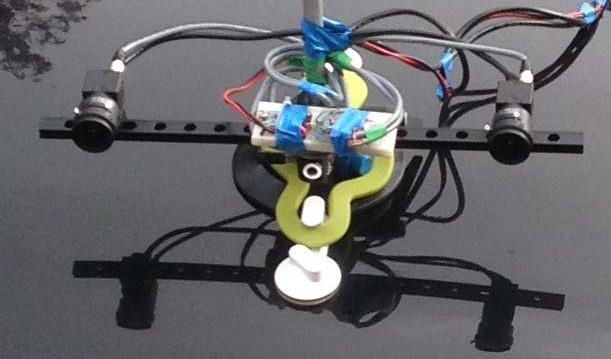
\includegraphics[height=6cm]{duas_cameras}
	\caption{Montagem com duas cameras}
	\label{fig:montagem_com_duas_cameras}
\end{figure}
Numa solução diferente, em \cite{Moazzam2013} é descrito um processo de deteção de buracos utilizando um sensor Kinect \footnote{https://developer.microsoft.com/en-us/windows/kinect} que só tem uma camera mas tem um sensor de infravermelhos para determinar a distância a que se encontra de um objeto. Esta solução tem resultados semelhantes aos de \cite{Zhang} e \cite{Chan2014} e para a sua implementação são necessários menos cálculos, uma vez que o software Kinect o faz de origem. Além disso, embora não seja apresentado, é de esperar que esta opção seja menos dispendiosa que as restantes.
\begin{figure}[htbp]
	\centering
	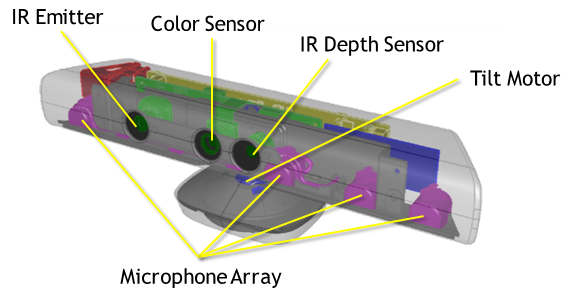
\includegraphics[height=6cm]{kinect}
	\caption{Sensor Kinect}
	\label{fig:sensor_kinect}
\end{figure}

\subsection{Camera vídeo com iluminação artificial}
\label{subsec: camera_video_com_iluminacao_artificial}
Apesar dos artigos apresentados nesta secção utilizarem também cameras, é interessante separá-los dos anteriores uma vez que a deteção dos buracos é feita de forma diferente, consoante a passagem pelo próprio buraco. Em \cite{Yu2011} e \cite{He2011} são projetadas linhas vermelhas no solo, perpendiculares à estrada, que deixam de ser retas sempre que existe uma perturbação na estrada. À medida que o sistema de deteção avança pela estrada, várias linhas são detetadas e é feito um mapeamento do buraco a analisar. A partir da análise da deformação das várias linhas é possível determinar a profundidade do buraco bem como as suas dimensões reais.

Não serão feitas comparações entre os casos já apresentados pois processamento de imagem não será o método a apresentar neste documento.

\subsection{Ultrassom}
\label{subsec: ultrassom}
Outra abordagem completamente diferente é a utilização de sensores ultrassom. É uma opção semelhante à que será tomada neste projeto na medida em que é quase obrigatório passar por um buraco para fazer a sua deteção, ao contrário da análise de imagens em que é possível evitá-los. Em \cite{Hegde2015} é mostrado um protótipo que permite a deteção de buracos através da análise do tempo de retorno de um ultrassom emitido e onde são determinados os valores a utilizar. \cite{Madli2015} é um projeto mais elaborado, em que uma montagem semelhante é utilizada num veículo e o conceito é testado em estradas reais. É possível elaborar uma relação entre os dois projetos em que \cite{Hegde2015} é um protótipo para \cite{Madli2015} visto existirem autores comuns a ambos e as suas referências se cruzarem.
\begin{figure}[hbtp]
	\centering
	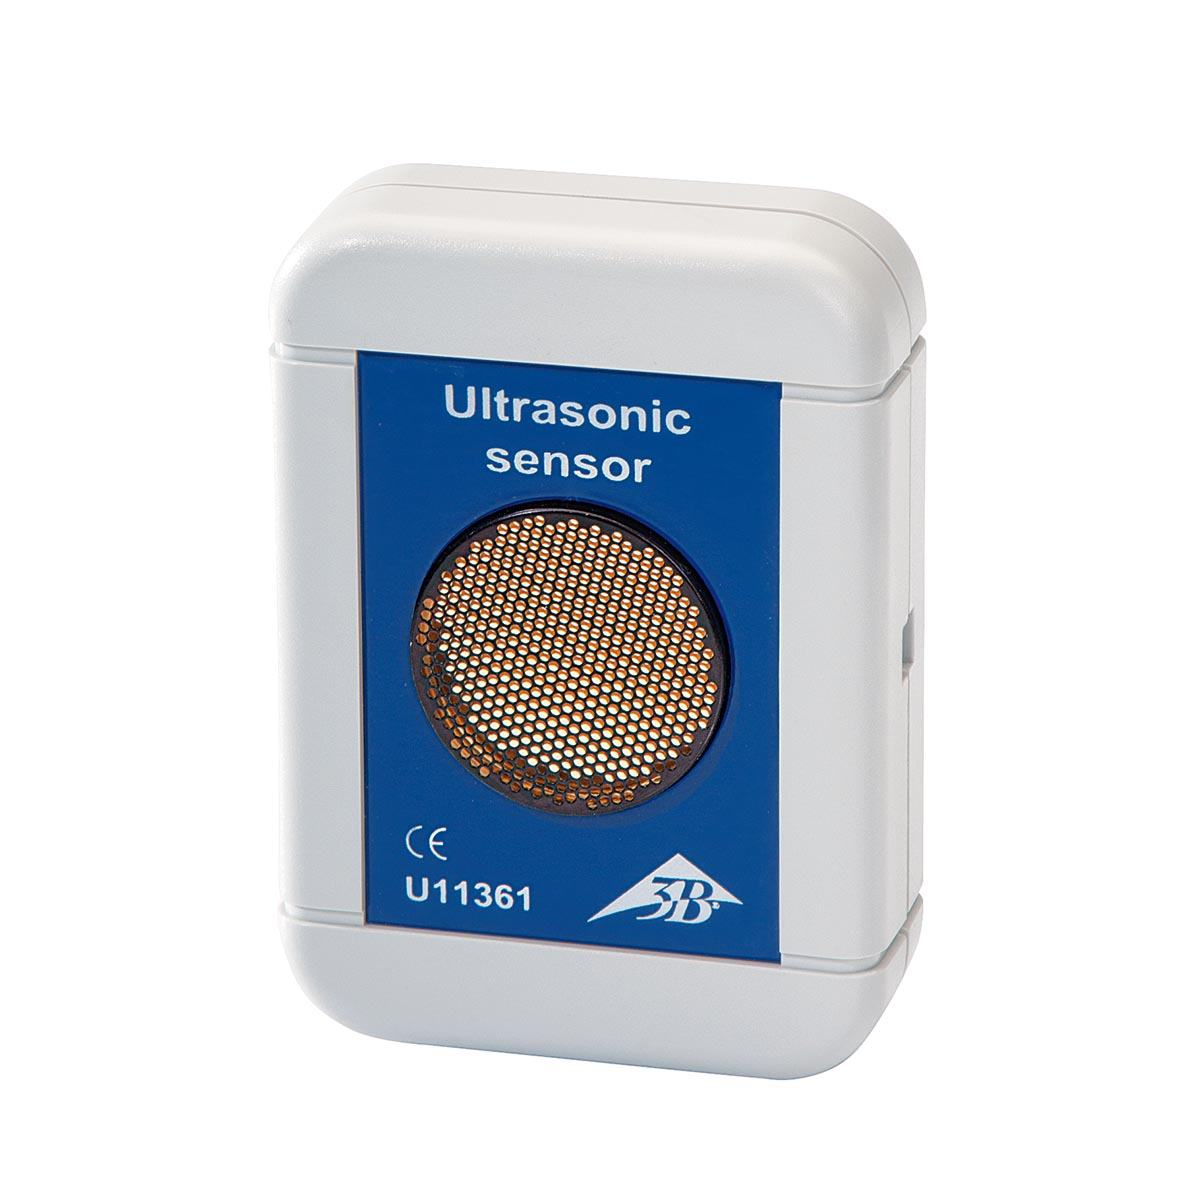
\includegraphics[height=6cm]{ultrassom}
	\caption{Sensor Ultrassom}
	\label{fig:sensor_ultrassom}
\end{figure}

\subsection{Acelerómetro}
\label{subsec: acelerometro}
Esta será a abordagem a ser utilizada e aquela em que os artigos analisados se mostram mais relevantes, devido à semelhança com o projeto que se pretende desenvolver. Em \cite{Mednis2011} é utilizado o acelerómetro do telefone e são apresentados vários algoritmos para a determinação do que é ou não um buraco na estrada. São também feitas algumas comparações sobre os resultados que diferentes telefones apresentam, dependendo do seu acelerómetro. No que diz respeito a \cite{Fouad}, é um documento semelhante ao anterior mas adiciona um giroscópio para melhor deteção de buracos. Embora os resultados apresentados sejam bons, terá que ser tido em conta o processamento extra necessário para a utilização dos dados do giroscópio que não parece adicionar muito mais sensibilidade ao sistema. Em \cite{Chen2011} foi criado um elemento que contém GPS e acelerómetro e ainda um microprocessador para processar os dados adquiridos. É um sistema muito bem construido e que apresenta vários resultados em estradas de diferentes condições mas poderá ser mais caro do que o pretendido desenvolver neste projeto. No artigo apresentado em \cite{Jang} é apresentada a comunicação entre vários veículos quanto à sua deteção de buracos. É uma ideia que poderá vir a ser implementada neste trabalho pelo que foi considerado um artigo bastante importante, apesar dos resultados apresentados serem relativos à comunicação e não  à deteção dos buracos especificamente. Por fim, é ainda de salientar o trabalho em \cite{Kattan2014} que apresenta uma metodologia semelhante à desejada tomar no que diz respeito à comunicação com uma base de dados mas com pouco desenvolvimento e uma curta fase de testes, pelo que será possível considerar que o trabalho a desenvolver será uma continuação deste.
\begin{figure}[hbtp]
	\centering
	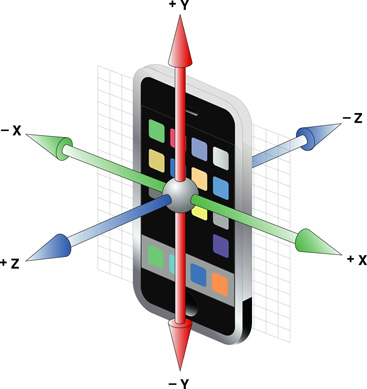
\includegraphics[height=6cm]{eixos_acelerometro}
	\caption{Direção dos eixos de um acelerómetro}
	\label{fig:direcao_dos_eixos_de_um_acelerometro}
\end{figure}

\section{Comparação de resultados} % (fold)
\label{sec:comapracao_de_resultados}

Comparando todos os artigos apresentados, é de notar que cada um tem os seus pontos fortes e fracos, como seria de esperar. Para o trabalho que será desenvolvido as qualidades mais importantes a ter em conta são o preço do material utilizado e também o tempo de processamento que o método consome. A tabela \ref{tab:comparacao_de_resultados_de_artigos} mostra as características que serão tidas em conta bem como quais as metodologias que as apresentam.

\begin{table}[htb]
\centering
\caption{Comparação de resultados de artigos}
\label{tab:comparacao_de_resultados_de_artigos}
\begin{tabular}{lcccc}
\multicolumn{1}{c}{} & \begin{tabular}[c]{@{}c@{}}Qualidade de \\ resultados\end{tabular} & \begin{tabular} [c] {@{}c@{}}Preço de \\ material \end{tabular} & \begin{tabular}[c]{@{}c@{}}Tempo de \\ processamento\end{tabular} & \begin{tabular}[c]{@{}c@{}}Processador \\ já incluído\end{tabular} \\
Camera vídeo & \cmark & \xmark & \xmark & \xmark \\
Camera + iluminação & \cmark& \xmark & \xmark & \xmark \\
Ultrassom & \cmark & \cmark & \cmark & \xmark \\
Acelerómetro & \cmark & \cmark & \cmark & \cmark
\end{tabular}
\end{table}

Desta forma, a utilização de um acelerómetro é a mais indicada. Dentro desta metodologia, ainda é possível fazer uma comparação dos vários artigos analisados e tirar algumas conclusões. Os resultados destas comparações são apresentados na tabela \ref{tab:comparacao_de_resultados_com_utilizacao_de_acelerometro}.

\begin{table}[htb]
\centering
\caption{Comparação de resultados com utilização de acelerómetro}
\label{tab:comparacao_de_resultados_com_utilizacao_de_acelerometro}
\begin{tabular}{lccccc}
\multicolumn{1}{c}{} & \begin{tabular}[c]{@{}c@{}}Acelerómetro\\ do telefone\end{tabular} & \begin{tabular}[c]{@{}c@{}}GPS do\\ telefone\end{tabular} & \begin{tabular}[c]{@{}c@{}}Giroscópio\\ do telefone\end{tabular} & \begin{tabular}[c]{@{}c@{}}Processador\\ do telefone\end{tabular} & \begin{tabular}[c]{@{}c@{}}Custos além\\ do telefone\end{tabular} \\
{\cite{Mednis2011}} & \cmark & \cmark & \xmark & \cmark & \xmark                              \\
{\cite{Fouad}} & \cmark & \cmark & \cmark & \cmark & \xmark                              \\
{\cite{Chen2011}} & \xmark & \xmark & \xmark & \xmark & \cmark
\end{tabular}
\end{table}

Embora os resultados dos trabalhos em que todos os componentes fazem parte do telefone sejam mais promissores em termos do preço dos materiais, a sua viabilidade é mais baixa, uma vez que um sistema que seja para o público em geral necessita de apresentar resultados consistentes, independentemente da situação e se o acelerómetro não estiver sempre no mesmo sítio (neste caso, o telefone) as leituras de cada buraco detetado são alteradas a cada passagem, dependendo do local em que o telefone se encontra, seja no bolso do casaco, no banco do veículo ou no seu \emph{tablier}. A utilização de GPS é obrigatória para que os buracos detetados possam ser localizados, sendo o sensor do telemóvel uma vantagem no que diz respeito aos custos, visto que a sua sensibilidade não necessita ser a mais alta, pois tratam-se de estradas e um erro de 5 metros é aceitável. Desta forma, a solução que será apresentada num projeto futuro terá que contar obrigatoriamente com um smartphone do utilizador, bem como um acelerómetro externo que será fixado no veículo, em princípio no amortecedor, algo que será ainda testado para obtenção de melhores resultados.

\section{Planeamento de trabalhos a desenvolver} % (fold)
\label{sec:planeamento_de_trabalhos_a_desenvolver}

De modo a estruturar melhor o desenvolvimento da dissertação, foi elaborado um planeamento para manter prazos e orientar mais facilmente os trabalhos necessários para o sucesso deste projeto, o qual pode ser visto na figura \ref{fig:planeamento_de_trabalhos_a_desenvolver}.

\begin{figure}[hbtp]
	\centering
	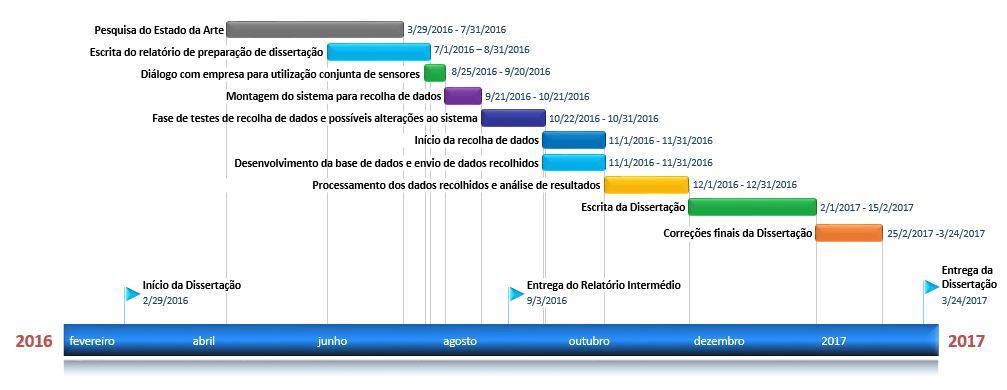
\includegraphics[height=22cm]{planeamento}
	\caption{Planeamento de trabalhos a desenvolver}
	\label{fig:planeamento_de_trabalhos_a_desenvolver}
\end{figure}